\documentclass[aspectratio=169]{beamer}
\usepackage{hyperref}
\usepackage[T1]{fontenc}
\usepackage[spanish]{babel}
\usepackage{csquotes}
\usepackage{tribhuvan}

\usepackage{latexsym,amsmath,xcolor,multicol,booktabs,calligra}
\usepackage{graphicx,pstricks,listings,stackengine}

\author{Rodrigo Pérez Rodríguez}
\title{Tecnologías Robóticas para la Discapacidad Intelectual}
\subtitle{Arquitecturas deliberativas e híbridas}
\date{}
\setbeamertemplate{date}{}

\AtBeginSection[]{
  \begin{frame}[plain]
    \vfill
    \begin{center}
      {\LARGE\bfseries \insertsectionhead}
    \end{center}
    \vfill
  \end{frame}
}
\AtBeginSubsection[]{}

\def\cmd#1{\texttt{\color{red}\footnotesize $\backslash$#1}}
\def\env#1{\texttt{\color{blue}\footnotesize #1}}
\definecolor{deepblue}{rgb}{0,0,0.5}
\definecolor{deepred}{rgb}{0.6,0,0}
\definecolor{deepgreen}{rgb}{0,0.5,0}
\definecolor{halfgray}{gray}{0.55}

\lstset{
    basicstyle=\ttfamily\small,
    keywordstyle=\bfseries\color{deepblue},
    emphstyle=\ttfamily\color{deepred},
    stringstyle=\color{deepgreen},
    numbers=left,
    numberstyle=\small\color{halfgray},
    rulesepcolor=\color{red!20!green!20!blue!20},
    frame=shadowbox,
}

\begin{document}

\begin{frame}
    \titlepage
\end{frame}

\begin{frame}
    \tableofcontents[sectionstyle=show,subsectionstyle=show/shaded/hide,subsubsectionstyle=show/shaded/hide]
\end{frame}

%=================================================
\section{De lo reactivo a lo deliberativo}
%=================================================

\begin{frame}{Por qué no basta con reaccionar}
\small
\begin{columns}[T,onlytextwidth]
  \begin{column}{0.58\textwidth}
    \begin{itemize}
      \item Lo reactivo funciona bien para reflejos y respuestas rápidas.
      \item En misiones largas aparecen límites: miopía temporal, oscilaciones y pérdida de contexto.
      \item La deliberación incorpora estado interno, objetivos y restricciones.
      \item Diseñar arquitectura implica decidir:
      \begin{itemize}
        \item qué sabe el robot,
        \item qué quiere lograr,
        \item y qué capacidades puede ejecutar.
      \end{itemize}
    \end{itemize}
  \end{column}
  \begin{column}{0.42\textwidth}
    \centering
    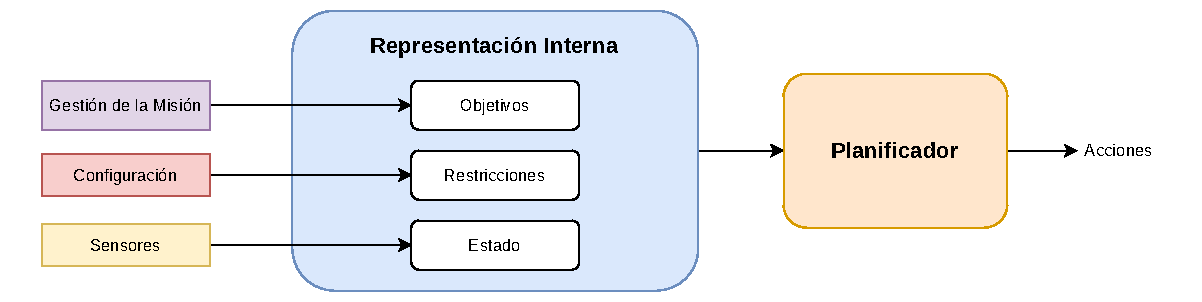
\includegraphics[width=0.97\linewidth,height=0.58\textheight,keepaspectratio]{images/tema_4/sistemas_deliberativos.pdf}
  \end{column}
\end{columns}
\end{frame}

\begin{frame}{Arquitecturas híbridas}
\small
\begin{columns}[T,onlytextwidth]
  \begin{column}{0.58\textwidth}
    \begin{itemize}
      \item No se trata de sustituir lo reactivo, sino de combinarlo con decisión de alto nivel.
      \item Reglas mínimas para que funcione:
      \begin{itemize}
        \item prioridades entre capas,
        \item flujo de información,
        \item autoridad para cancelar o preemptar acciones.
      \end{itemize}
      \item Se reparte el sistema por escalas temporales:
      \begin{itemize}
        \item ms: seguridad y control,
        \item s: ejecución de tareas,
        \item min: misión y planificación.
      \end{itemize}
    \end{itemize}
  \end{column}
  \begin{column}{0.42\textwidth}
    \centering
    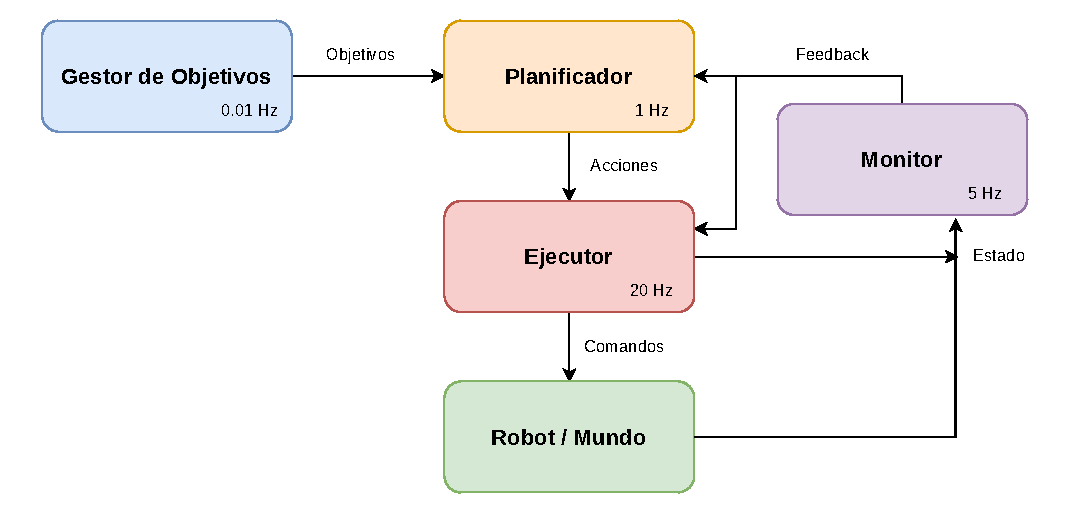
\includegraphics[width=0.97\linewidth,height=0.58\textheight,keepaspectratio]{images/tema_4/responsabilidades.pdf}
  \end{column}
\end{columns}
\end{frame}

\begin{frame}{Receta de diseño}
\small
\begin{itemize}
  \item Definir horizonte temporal de cada decisión (rápida, media, lenta).
  \item Fijar objetivos verificables y restricciones de seguridad.
  \item Modelar capacidades como servicios con contrato: entradas, feedback, resultado y fallos.
  \item Diseñar supervisión: qué monitorizar, cuándo recuperar y cuándo replanificar.
  \item Establecer arbitraje entre capas para evitar bloqueos y oscilaciones.
\end{itemize}
\end{frame}

%=================================================
\section{Arquitecturas en capas}
%=================================================

\begin{frame}{Misión, tarea y capacidad}
\small
\begin{columns}[T,onlytextwidth]
  \begin{column}{0.58\textwidth}
    \begin{itemize}
      \item \textbf{Misión:} decide qué hacer y con qué prioridades.
      \item \textbf{Tarea:} orquesta secuencias, recuperaciones y progreso.
      \item \textbf{Capacidad:} ejecuta acciones concretas de forma segura.
      \item La separación por capas mejora coherencia, reutilización y depuración.
      \item Hacia abajo bajan objetivos; hacia arriba suben resultados y razones de fallo.
    \end{itemize}
  \end{column}
  \begin{column}{0.42\textwidth}
    \centering
    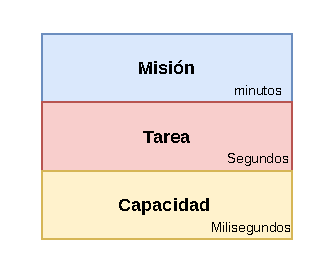
\includegraphics[width=0.97\linewidth,height=0.58\textheight,keepaspectratio]{images/tema_4/mision_tarea_capacidad.pdf}
  \end{column}
\end{columns}
\end{frame}

\begin{frame}{Contratos entre capas}
\small
\begin{columns}[T,onlytextwidth]
  \begin{column}{0.58\textwidth}
    \begin{itemize}
      \item La misión no debe hablar directamente con sensores o actuadores.
      \item La capacidad no debería conocer el objetivo global de la misión.
      \item Cada frontera necesita contratos explícitos:
      \begin{itemize}
        \item precondiciones,
        \item parámetros,
        \item feedback,
        \item cancelación y timeout.
      \end{itemize}
      \item Esto reduce acoplamientos y facilita evolución del sistema.
    \end{itemize}
  \end{column}
  \begin{column}{0.42\textwidth}
    \centering
    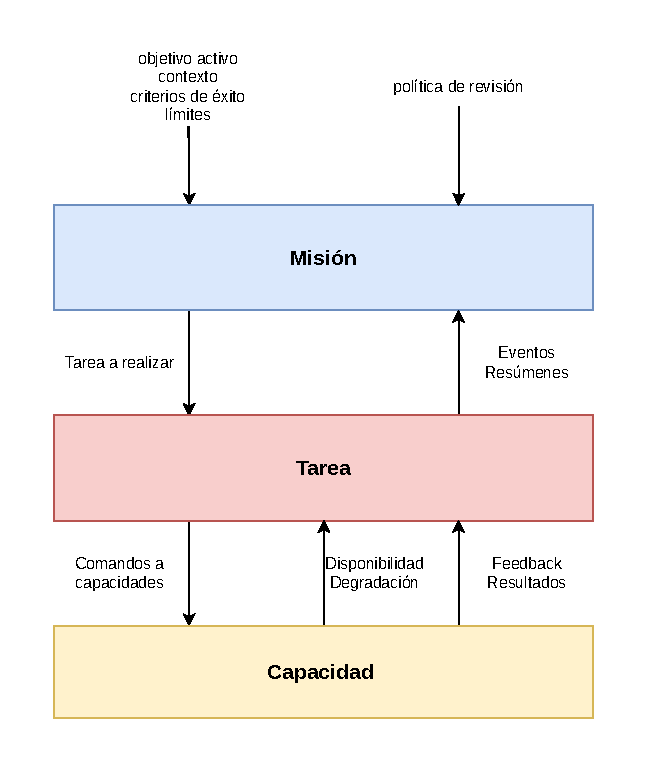
\includegraphics[width=0.97\linewidth,height=0.58\textheight,keepaspectratio]{images/tema_4/mision_tarea_capacidad_ext.pdf}
  \end{column}
\end{columns}
\end{frame}

\begin{frame}{Subsumption y arbitraje reactivo}
\small
\begin{columns}[T,onlytextwidth]
  \begin{column}{0.58\textwidth}
    \begin{itemize}
      \item Capas reactivas en paralelo compiten por el control.
      \item El arbitraje se basa en prioridad por supresión/inhibición.
      \item Ventaja: respuestas robustas ante eventos rápidos.
      \item Límite: escalar a misiones largas es difícil sin estado explícito.
      \item Integración recomendada: reflejos en capacidades, intención global en misión/tarea.
    \end{itemize}
  \end{column}
  \begin{column}{0.42\textwidth}
    \centering
    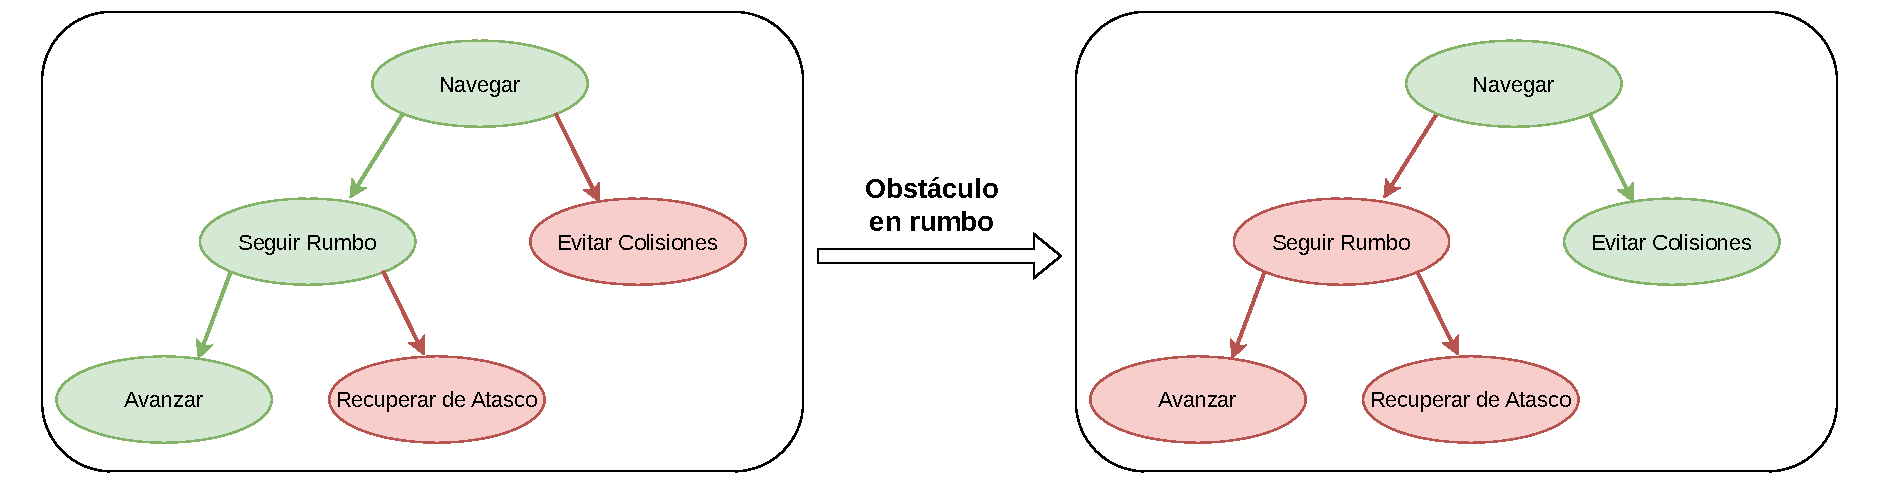
\includegraphics[width=0.97\linewidth,height=0.58\textheight,keepaspectratio]{images/tema_4/subsumption.pdf}
  \end{column}
\end{columns}
\end{frame}

%=================================================
\section{Modelos del mundo}
%=================================================

\begin{frame}{Modelo del mundo como frontera}
\small
\begin{columns}[T,onlytextwidth]
  \begin{column}{0.58\textwidth}
    \begin{itemize}
      \item Integra percepciones en conocimiento consultable para decidir.
      \item Debe mantener coherencia espacial y temporal.
      \item Incluye estimación, asociación de datos y caducidad de la información.
      \item También representa incertidumbre y confianza.
    \end{itemize}
  \end{column}
  \begin{column}{0.42\textwidth}
    \centering
    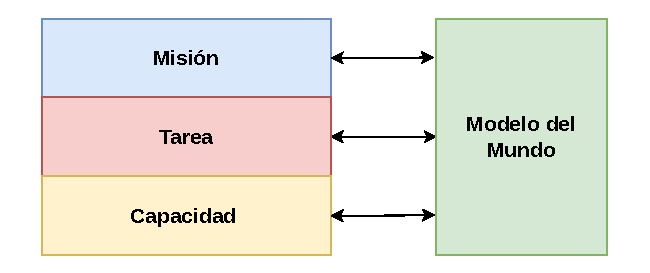
\includegraphics[width=0.97\linewidth,height=0.58\textheight,keepaspectratio]{images/tema_4/mision_tarea_capacidad_world_model.pdf}
  \end{column}
\end{columns}
\end{frame}

\begin{frame}{Consultas orientadas a decisión}
\small
\begin{itemize}
  \item Publicar datos no es suficiente: hay que ofrecer consultas útiles para misión y tarea.
  \item Ejemplos: dónde estoy, qué hay cerca, qué entidad está activa, qué riesgo existe.
  \item La deliberación se activa por eventos relevantes, no por todo cambio de sensor.
  \item Regla práctica: modelar explícitamente lo que realmente cambia decisiones.
\end{itemize}
\end{frame}

\begin{frame}{Diseños habituales de modelo del mundo}
\small
\begin{columns}[T,onlytextwidth]
  \begin{column}{0.56\textwidth}
    \begin{itemize}
      \item \textbf{Servidor central:} un único punto integra y responde.
      \item \textbf{Vistas federadas:} cada subsistema aporta su estimación.
      \item \textbf{Modelo dual:} capa geométrica + capa simbólica para planificación.
      \item No hay diseño universal: depende del dominio, carga y requisitos de trazabilidad.
    \end{itemize}
  \end{column}
  \begin{column}{0.44\textwidth}
    \centering
    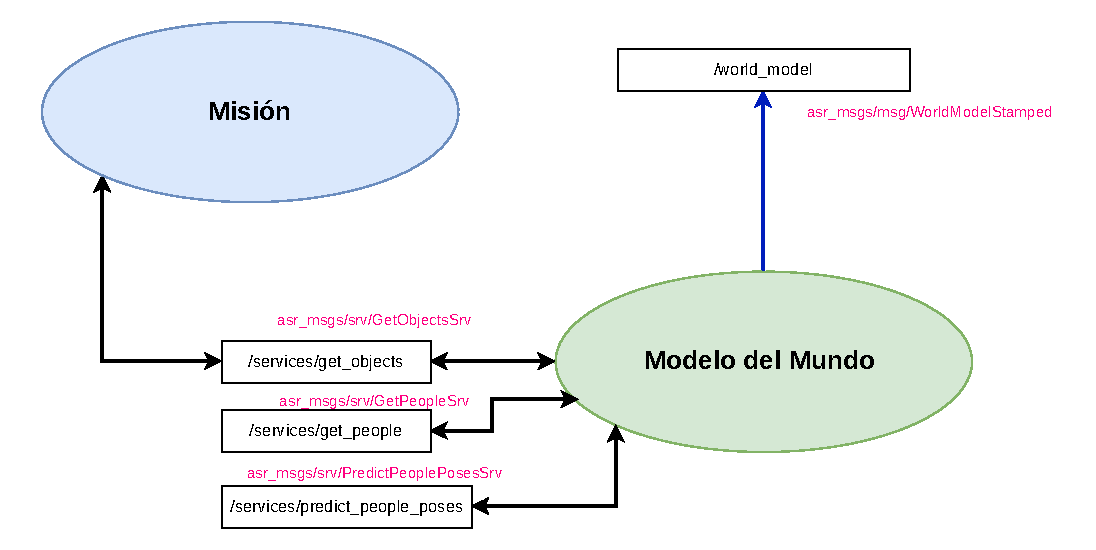
\includegraphics[width=0.97\linewidth,height=0.25\textheight,keepaspectratio]{images/tema_4/world_model_interfaces.pdf}
    \par\vspace{0.01\textheight}
    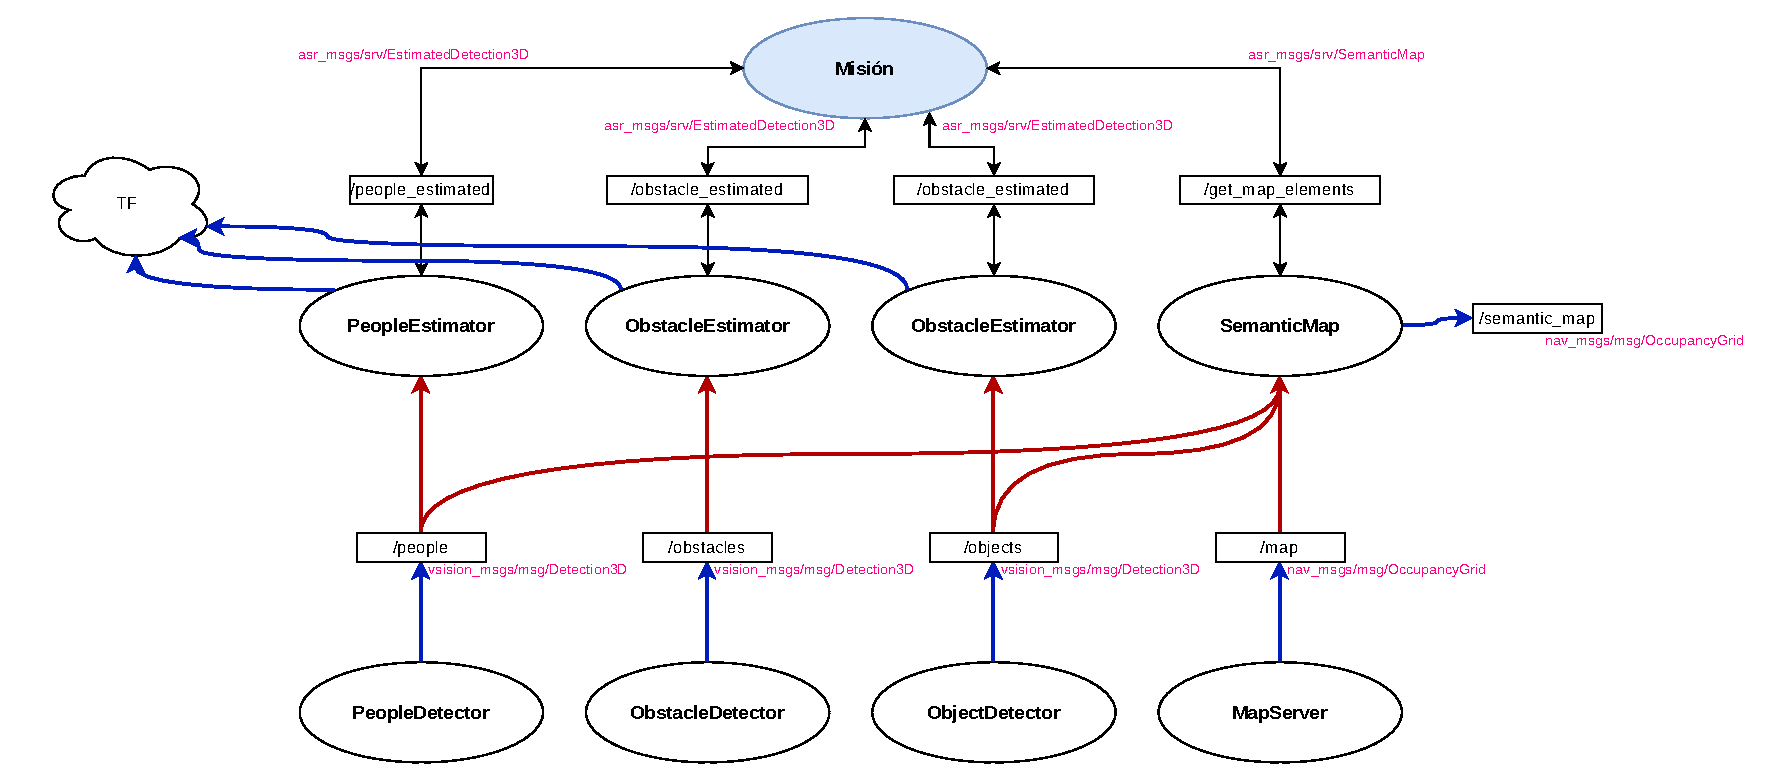
\includegraphics[width=0.97\linewidth,height=0.25\textheight,keepaspectratio]{images/tema_4/world_model_2.pdf}
  \end{column}
\end{columns}
\end{frame}

%=================================================
\section{Aplicación en ROS 2}
%=================================================

\begin{frame}{Mapeo a un grafo de ROS 2}
\small
\begin{columns}[T,onlytextwidth]
  \begin{column}{0.58\textwidth}
    \begin{itemize}
      \item La arquitectura se concreta en un grafo de nodos y comunicaciones.
      \item Roles típicos:
      \begin{itemize}
        \item misión como supervisor,
        \item tarea como orquestador,
        \item capacidades como proveedores.
      \end{itemize}
      \item Interfaces típicas:
      \begin{itemize}
        \item acciones para actividades largas,
        \item topics para estado continuo,
        \item servicios para consultas puntuales.
      \end{itemize}
    \end{itemize}
  \end{column}
  \begin{column}{0.42\textwidth}
    \centering
    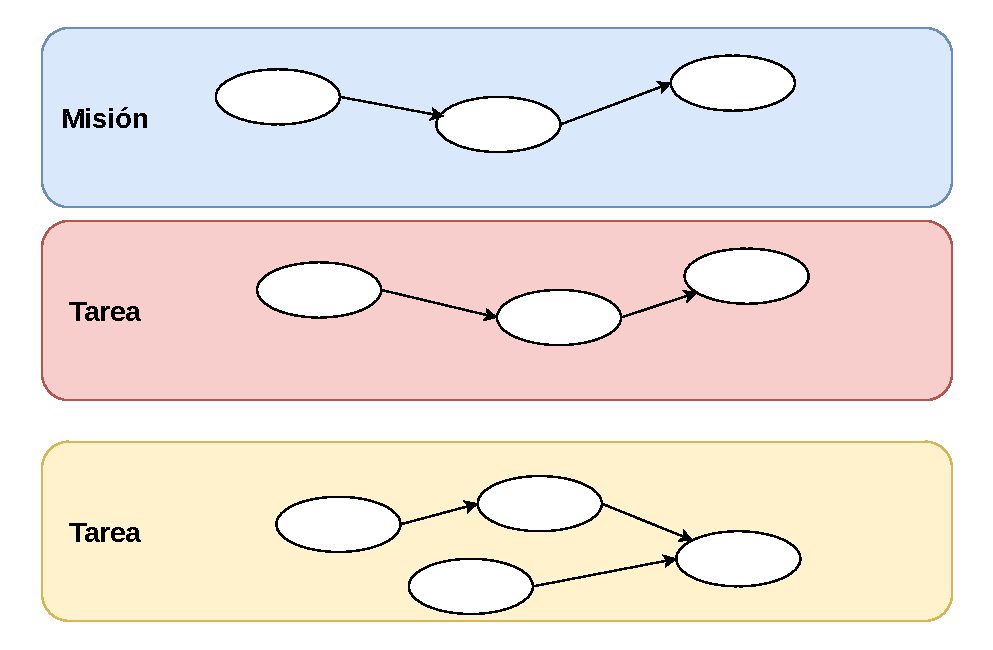
\includegraphics[width=0.97\linewidth,height=0.58\textheight,keepaspectratio]{images/tema_4/mision_tarea_capacidad_ros_pre.pdf}
  \end{column}
\end{columns}
\end{frame}

\begin{frame}{Tarea y capacidades en ROS 2}
\small
\begin{columns}[T,onlytextwidth]
  \begin{column}{0.58\textwidth}
    \begin{itemize}
      \item La tarea combina capacidades y gestiona contexto de ejecución.
      \item Las capacidades exponen progreso, resultado, cancelación y diagnóstico.
      \item Es habitual usar árboles de comportamiento (BT) para orquestación robusta.
      \item Ejemplos reales: navegación y manipulación como subsistemas gobernables.
    \end{itemize}
  \end{column}
  \begin{column}{0.42\textwidth}
    \centering
    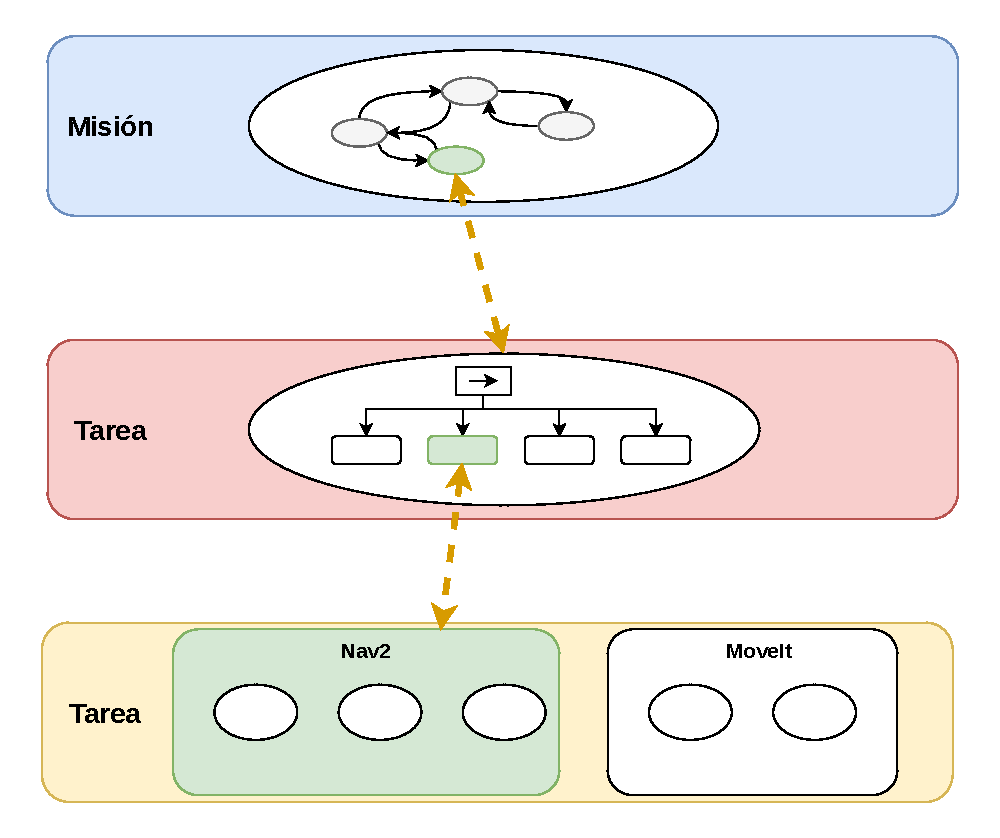
\includegraphics[width=0.97\linewidth,height=0.58\textheight,keepaspectratio]{images/tema_4/mision_tarea_capacidad_ros.pdf}
  \end{column}
\end{columns}
\end{frame}

\begin{frame}{Misión: FSM o planificador}
\small
\begin{columns}[T,onlytextwidth]
  \begin{column}{0.58\textwidth}
    \begin{itemize}
      \item \textbf{FSM:} útil cuando el conjunto de situaciones es acotado.
      \item \textbf{Planificador:} útil cuando hay objetivos, recursos y restricciones complejas.
      \item En ambos casos la misión debe:
      \begin{itemize}
        \item priorizar,
        \item cancelar/preemptar,
        \item justificar decisiones.
      \end{itemize}
    \end{itemize}
  \end{column}
  \begin{column}{0.42\textwidth}
    \centering
    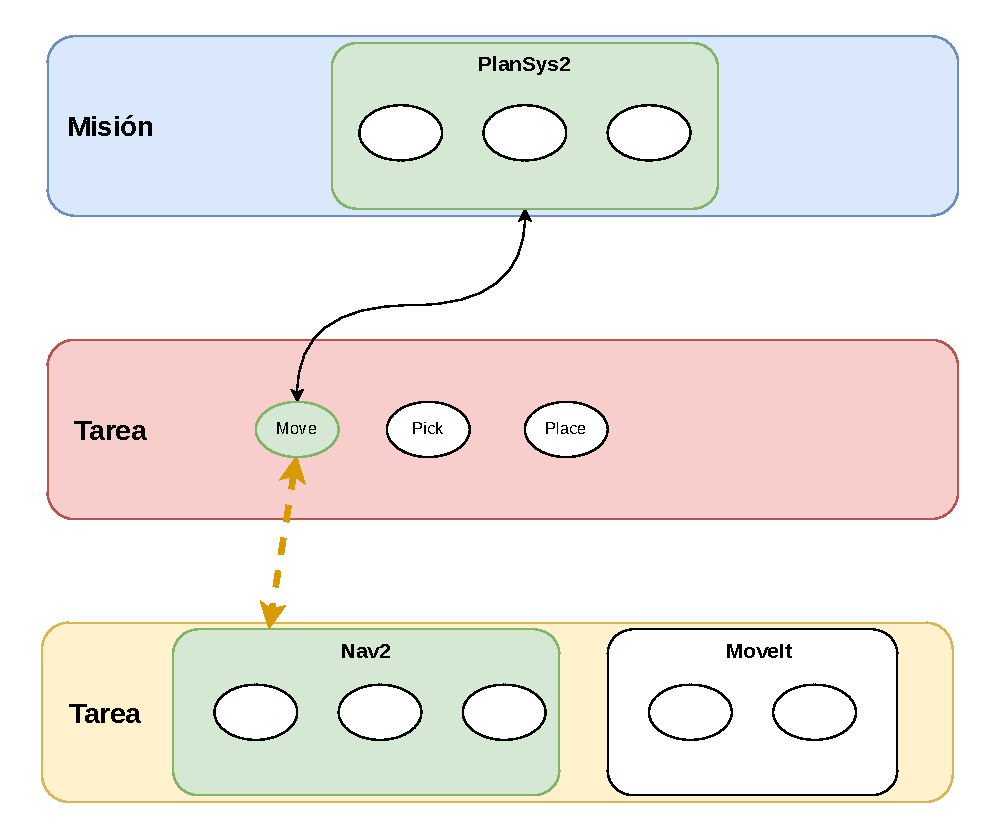
\includegraphics[width=0.97\linewidth,height=0.58\textheight,keepaspectratio]{images/tema_4/mision_tarea_capacidad_ros_plansys.pdf}
  \end{column}
\end{columns}
\end{frame}

\begin{frame}{Lifecycle Nodes y operación segura}
\small
\begin{columns}[T,onlytextwidth]
  \begin{column}{0.58\textwidth}
    \begin{itemize}
      \item Un lifecycle node separa crear de activar: permite arranques ordenados.
      \item Estados típicos: unconfigured, inactive, active.
      \item Transiciones controladas: configure, activate, deactivate, cleanup.
      \item Ventaja práctica: degradar o recuperar módulos sin reiniciar todo el sistema.
    \end{itemize}
  \end{column}
  \begin{column}{0.42\textwidth}
    \centering
    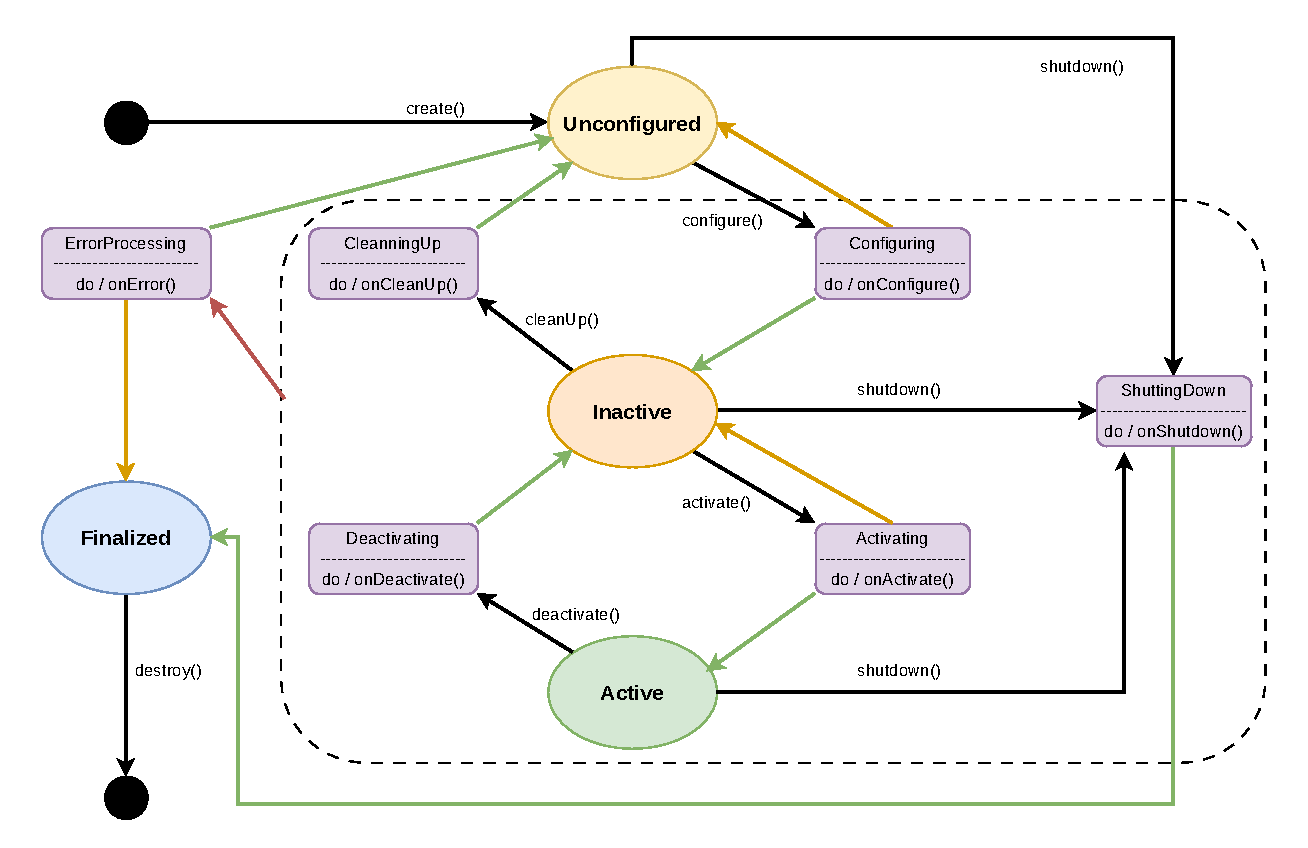
\includegraphics[width=0.97\linewidth,height=0.58\textheight,keepaspectratio]{images/tema_4/LifeCycleNode.pdf}
  \end{column}
\end{columns}
\end{frame}

\begin{frame}{Conclusiones}
\small
\begin{itemize}
  \item Las arquitecturas híbridas combinan rapidez reactiva con coherencia deliberativa.
  \item Separar misión, tarea y capacidad mejora mantenibilidad y escalabilidad.
  \item El modelo del mundo es clave para decisiones trazables y seguras.
  \item En ROS 2, contratos + TF + ciclo de vida hacen viable esta arquitectura en sistemas reales.
\end{itemize}
\end{frame}

\begin{frame}
  \centering
  \Large Preguntas
\end{frame}

\end{document}
